% Hardware Design Chapter

\providecommand{\capstack}{}
\renewcommand{\capstack}[1]{\begin{tabular}[c]{@{}l@{}}#1\end{tabular}}

\chapter{Hardware Design}
\label{chap:hardware_design}

This chapter details the hardware design focused on ensuring that the prototype functions correctly and to an adequate standard in its physical realisation by justifying the hardware selected. A primary concern was minimising the noise coupled into the measurement from other parts of the system, such as the Wi-Fi transmissions, the display, and reads and writes to the SD card. This was addressed through decoupling (Section~\ref{sec:hw_caps}), a ferrite bead on
the analog supply (Section~\ref{sec:hw_ferrite}), and the separation of the analog and
digital grounds (Section~\ref{sec:hw_ground}).

\section{AFE Requirements}
\label{sec:requirements}
 
The research group at the University of Johannesburg \cite{ebrahim_dpv_conditions} specified the measurement method as well as the parameters that the OpenStat should fulfil. The operating requirements are listed in Table~\ref{tab:req_dpv}. The same parameters are used on the PalmSens4
reference instrument in Chapter~\ref{chap:testing}.
 
\begin{table}[H]
  \centering
  \caption{Target DPV operating conditions and the requirements they impose.}
  \label{tab:req_dpv}
  \begin{tabularx}{\textwidth}{@{}l l >{\raggedright\arraybackslash}X@{}}
    \toprule
    \textbf{Parameter} & \textbf{Value} & \textbf{Requirement on the device} \\
    \midrule
    Potential window  & \SIrange{0.8}{1.3}{\volt} &
      Potential covers \SIrange{0.8}{1.325}{\volt}, including the pulse \\
    Step potential    & \SI{5}{\milli\volt} &
      DAC LSB $\leq$ \SI{1}{\milli\volt}, each level within
      $\pm 0.5$\,LSB  \\
    Pulse amplitude   & \SI{25}{\milli\volt} &
      $25\pm$\SI{1}{\milli\volt} \\
    Pulse time        & \SI{50}{\milli\second} &
      Timing error changes the sampled current by $\leq$ \SI{2}{\percent} \\
    Interval time     & \SI{0.5}{\second} &
      \SI{0.5}{\second} $\pm$ \SI{1}{\percent} per step, held over the full scan \\
    \midrule
    Current range     & $\pm\SI{750}{\micro\ampere}$ &
      No saturation at $\pm\SI{750}{\micro\ampere}$, gain error
      $\leq$ \SI{1}{\percent} per RTIA range after calibration \\
    \bottomrule
  \end{tabularx}
\end{table}

The AD5941 was specified at the start of the project and meets these requirements on a single chip, with \SI{0.54}{\milli\volt} DAC steps and eight TIA gain ranges covering $\pm\SI{750}{\micro\ampere}$ \cite{ad5941_ds}. Appendix~\ref{app:afe_choice} compares it with the alternatives.

\section{System Requirements}

The table below details the requirements that the OpenStat must meet.
\begin{table}[h]
\centering
\caption{System requirements.}
\label{tab:requirements_whole_sys}
\begin{tabularx}{\textwidth}{l X X}
\toprule
ID & Requirement & Rationale \\
\midrule
\multicolumn{3}{l}{\textit{Processing and memory}} \\
R1 & Buffer a complete scan in memory & Samples are written to storage only after the scan finishes \\
R2 & At least two SPI buses available for peripherals & One dedicated to the AD5941, one shared by the display and SD card \\
R3 & Dedicated GPIO for the AD5941, display, SD card and user inputs & All peripherals connected without sharing control lines \\
\midrule
\multicolumn{3}{l}{\textit{Display and storage}} \\
R4 & Colour display with an SPI or I\textsuperscript{2}C interface & Compatible with the microcontroller \\
R5 & Display fits in landscape orientation & Handheld form factor \\
R6 & At least 100 horizontal pixels & One pixel per point of a 100-point scan \\
R7 & Non-volatile storage & Field measurements accessed later \\
\midrule
\multicolumn{3}{l}{\textit{User interface}} \\
R8 & Standalone operation without a computer & Scan parameters set and scans started in the field \\
\midrule
\multicolumn{3}{l}{\textit{Power}} \\
R9 & Battery powered & Portable field use \\
R10 & Rechargeable from USB & No battery replacement needed \\
R11 & Regulated supply over discharge range & Cell voltage varies from 3.0 to 4.2\,V \\
R12 & At least 8\,h of operation per charge & 8-hour working day \\
\bottomrule
\end{tabularx}
\end{table}

To start implementing the above requirements, the microcontroller is specified next.

\section{Microcontroller}
\label{sec:hw_mcu}

The microcontroller must drive the AD5941 on a dedicated SPI bus while a second bus serves the display and SD card (R2), buffer a complete scan (R1), and serve the web interface over Wi-Fi without a companion app (Objective~4). The ESP32 family was chosen, as it is the MCU used by the  designs surveyed in Table~\ref{tab:design_comparison} that has native Wi-Fi that Objective~4 requires. Its newer ESP32-S3 member was used, on a development board based on the ESP32-S3-WROOM-2-N32R16V module \cite{esp32s3_wroom2_ds}. This provides the two general-purpose SPI controllers needed for R2, and its \SI{16}{\mega\byte} of PSRAM is far more than one scan requires, but leaves room to buffer several scans and the web assets.

\section{PCB Component Placement and Layout}
\label{sec:hw_afe}

The key to low noise in the AD5941 is sufficient filtering and decoupling,
together with correct component placement. The rules followed when selecting
the decoupling capacitors were taken from the Analog Devices MT-101 tutorial
\cite{adi_mt101}. Finally, a ferrite bead is placed in series with the
supply pin. This keeps external high-frequency noise away from the IC and
prevents internally generated noise from affecting the rest of the system \cite{eco2016ferrite}.

\providecommand{\capstack}[1]{\begin{tabular}[t]{@{}l@{}}#1\end{tabular}}
 
\subsection{Capacitor Choices}
\label{sec:hw_caps}
 
The capacitors around the AD5941 can be separated into two groups, decoupling the external supply pins and connecting internal nodes with the IC. Table~\ref{tab:hw_caps} summarises the capacitor choices for their respective roles. The supply-pin values follow the MT-101
two-tier convention \cite{adi_mt101} and are checked against a target supply
impedance, while the internal-node values follow the datasheet
\cite{ad5941_ds}. The full derivations for capacitor choices are given in
Appendix~\ref{appen:hw_caps}.
 
\begin{table}[H]
  \centering
  \small
  \caption{Capacitors around the AD5941, grouped by the reasoning behind
    each value.}
  \label{tab:hw_caps}
  \renewcommand\tabularxcolumn[1]{m{#1}}
  \begin{tabularx}{\textwidth}{@{}l l >{\raggedright\arraybackslash}X@{}}
    \toprule
    \textbf{Pin} & \textbf{Value} & \textbf{Role and justification} \\
    \midrule
    % --- Group 1: high-frequency supply decoupling ---------------------
    \capstack{DVDD (6), $\times 2$ \\ IOVDD (26) \\ AVDD (30) \\ AVDD (41)}
      & \SI{100}{\nano\farad}
      & \textit{High-frequency supply decoupling.} No datasheet value given, so one
        ceramic capacitor per supply pin, as per MT-101 \cite{adi_mt101}. Stays
        below the \SI{1}{\ohm} target impedance to beyond
        \SI{100}{\mega\hertz} (Eq.~\eqref{eq:hw_esl_100mhz})
        \cite{smith1999pds}. \\
    \midrule
    % --- Group 2: bulk decoupling --------------------------------------
    AVDD (30) & \SI{10}{\micro\farad}
      & \textit{Bulk decoupling.} Second tier of MT-101 \cite{adi_mt101}.
        Meets the \SI{1}{\ohm} target above \SI{15.9}{\kilo\hertz}
        (Eq.~\eqref{eq:hw_fmin}) and forms an LC filter with the ferrite bead
        (Section~\ref{sec:hw_ferrite}). \\
    \midrule
    % --- Group 3: references and internal LDOs, 470 nF -----------------
    \capstack{\texttt{VREF\_2V5} (4) \\ \texttt{VBIAS\_CAP} (31) \\
              \texttt{DVDD\_REG\_1V8} (14) \\ \texttt{AVDD\_REG} (5)}
      & \SI{470}{\nano\farad}
      & \textit{Reference and internal LDO decoupling.} Datasheet value
        \cite[pp.~11, 20--21]{ad5941_ds}, set by the stability of on-chip
        buffers and regulators \cite{rinconmora2009ldo}. No value is given
        for \texttt{AVDD\_REG}, so it is matched to \texttt{DVDD\_REG\_1V8}. \\
    \midrule
    % --- Group 4: ADC reference -----------------------------------------
    \texttt{VREF\_1V82} (43) & \SI{4.7}{\micro\farad}
      & \textit{ADC reference reservoir.} The datasheet recommends
        \SI{4.7}{\micro\farad} \cite[p.~19]{ad5941_ds} but tests at
        \SI{0.47}{\micro\farad} \cite[p.~11]{ad5941_ds}. The larger value was
        chosen as the more conservative. \\
    \midrule
    % --- Group 5: LP DAC outputs -----------------------------------------
    \capstack{\texttt{VBIAS0} (8) \\ \texttt{VZERO0} (9)}
      & \SI{100}{\nano\farad}
      & \textit{Low-power DAC output noise filter.} Datasheet value
        \cite[p.~20]{ad5941_ds}. \\
    \midrule
    % --- Group 6: reset --------------------------------------------------
    \texttt{RESET} (22) & \SI{100}{\nano\farad}
      & \textit{Reset debounce.} With the \SI{10}{\kilo\ohm} pull-up,
        $\tau = \SI{1}{\milli\second} \gg \SI{1}{\micro\second}$ minimum
        reset pulse \cite[p.~14]{ad5941_ds}. \\
    \bottomrule
  \end{tabularx}
\end{table}

Together, the two tiers of supply capacitors hold AVDD below the
\SI{1}{\ohm} target from about \SI{16}{\kilo\hertz} to beyond
\SI{100}{\mega\hertz}, which keeps supply noise below one LSB at the ADC
reference. Noise arriving from the rest of the board is
blocked separately by the ferrite bead.
% OPTIONAL -- uncomment only if the 220 ohm 0.1 % resistor in the BOM is the AD5941's RCAL:
% A \SI{220}{\ohm}, \SI{0.1}{\percent} resistor is fitted as RCAL \cite{ad5941_ds}; the calibration in this project used external resistors instead (Section~\ref{sec:rtia_cal}).
 
\subsection{Ferrite Bead}
\label{sec:hw_ferrite}
AVDD shares the 3.3\,V rail with the ESP32-S3, display and SD card. These components
place noise on the rail from tens of kilohertz to hundreds of megahertz \cite{eco2016ferrite}. This noise comes
from the SPI clocks, regulator ripple and current bursts. A ferrite bead in series with
AVDD forms a low-pass filter with the AVDD decoupling capacitors of
Section~\ref{sec:hw_caps}, and over its resistive band it dissipates
this noise as heat instead of reflecting it~\cite{eco2016ferrite}. A bead was
preferred over a separate regulator for AVDD because it adds a single small, inexpensive
part that is most effective at high frequencies. The W\"urth Elektronik 74279204 was chosen for its impedance of 600\,$\Omega$ at 100\,MHz, with a rated
current of 200\,mA and a maximum DC resistance $R_\mathrm{DC}$ of
0.35\,$\Omega$~\cite{wurth74279204}.

The bead operates far from the point where DC current degrades its filtering. Impedance
curves from the datasheet are measured at zero bias, and under load the core saturates
and the inductance falls. Therefore, the bead should operate at no more than about 20\,\%
of its rated current~\cite{eco2016ferrite}. The worst-case AVDD current of about
10\,mA is 5\,\% of the rating, so the datasheet impedance applies. The resulting 3.5\,mV
drop uses 1.2\,\% of the 0.3\,V allowed between AVDD and DVDD~\cite[p.~7]{ad5941_ds}.

The primary risk with ferrite beads is resonance. Below its crossover frequency the bead
is almost purely inductive, and it resonates with the decoupling capacitors. An
underdamped resonance amplifies noise instead of attenuating it, which is called
peaking~\cite{eco2016ferrite}. For the series RLC filter,
\begin{equation}
f_0 = \frac{1}{2\pi\sqrt{L_\mathrm{bead}C}} \approx 50\,\mathrm{kHz}, \qquad
Q = \frac{1}{R_\mathrm{DC}}\sqrt{\frac{L_\mathrm{bead}}{C}} \approx 0.90,
\end{equation}
with $C = 10\,\mu$F, the AVDD bulk capacitor of Table~\ref{tab:hw_caps}, and an assumed
$L_\mathrm{bead} \approx 1\,\mu$H, consistent with the 600\,$\Omega$ rating at 100\,MHz.
A second-order filter peaks for $Q > 1/\sqrt{2}$~\cite{c2}, so the response rises by
about 0.7\,dB near 30\,kHz, which is negligible.

It is the 10\,$\mu$F bulk capacitor that keeps the resonance well damped. The large capacitor lowers $\sqrt{L/C}$ until the bead's own series resistance
is sufficient to damp the filter, so the bulk capacitor also serves to damp the bead.

At high frequencies the filter performs as intended. At 100\,MHz the bead's 600\,$\Omega$
and the 0.63\,$\Omega$ of the local 100\,nF capacitors (Eq.~(\ref{eq:hw_esl_100mhz})) form a
divider that attenuates noise by about
$20\log_{10}(0.63/600) \approx -60$\,dB.

\subsection{Analog and Digital Ground}
\label{sec:hw_ground}

The PCB carries two types of signals, analog and digital, whose requirements
conflict. The AD5941 AFE measures small Faradaic currents, so any disturbance
appears as a measurement error. In contrast, the ESP32-S3, the display and the
user inputs are digital. This means that they draw fast pulses of current at set logic levels,
and that current must return to its source through ground. A ground plane is
not ideal for this as it has a small resistance and inductance, so a rapidly changing
current induces a voltage according to $v = L\,\mathrm{d}i/\mathrm{d}t$. If
the analog and digital circuits share the same ground return, this voltage is
added to the analog reference and the digital switching noise is superimposed
on the measured signal \cite{adi_mt031}.

\begin{wrapfigure}{r}{0.25\textwidth}
    \vspace{-\baselineskip}
    \caption{PCB copper layout, with the digital region at the top and the analog region at the bottom.}
    \label{fig:hw_ground_partition}
    \centering
    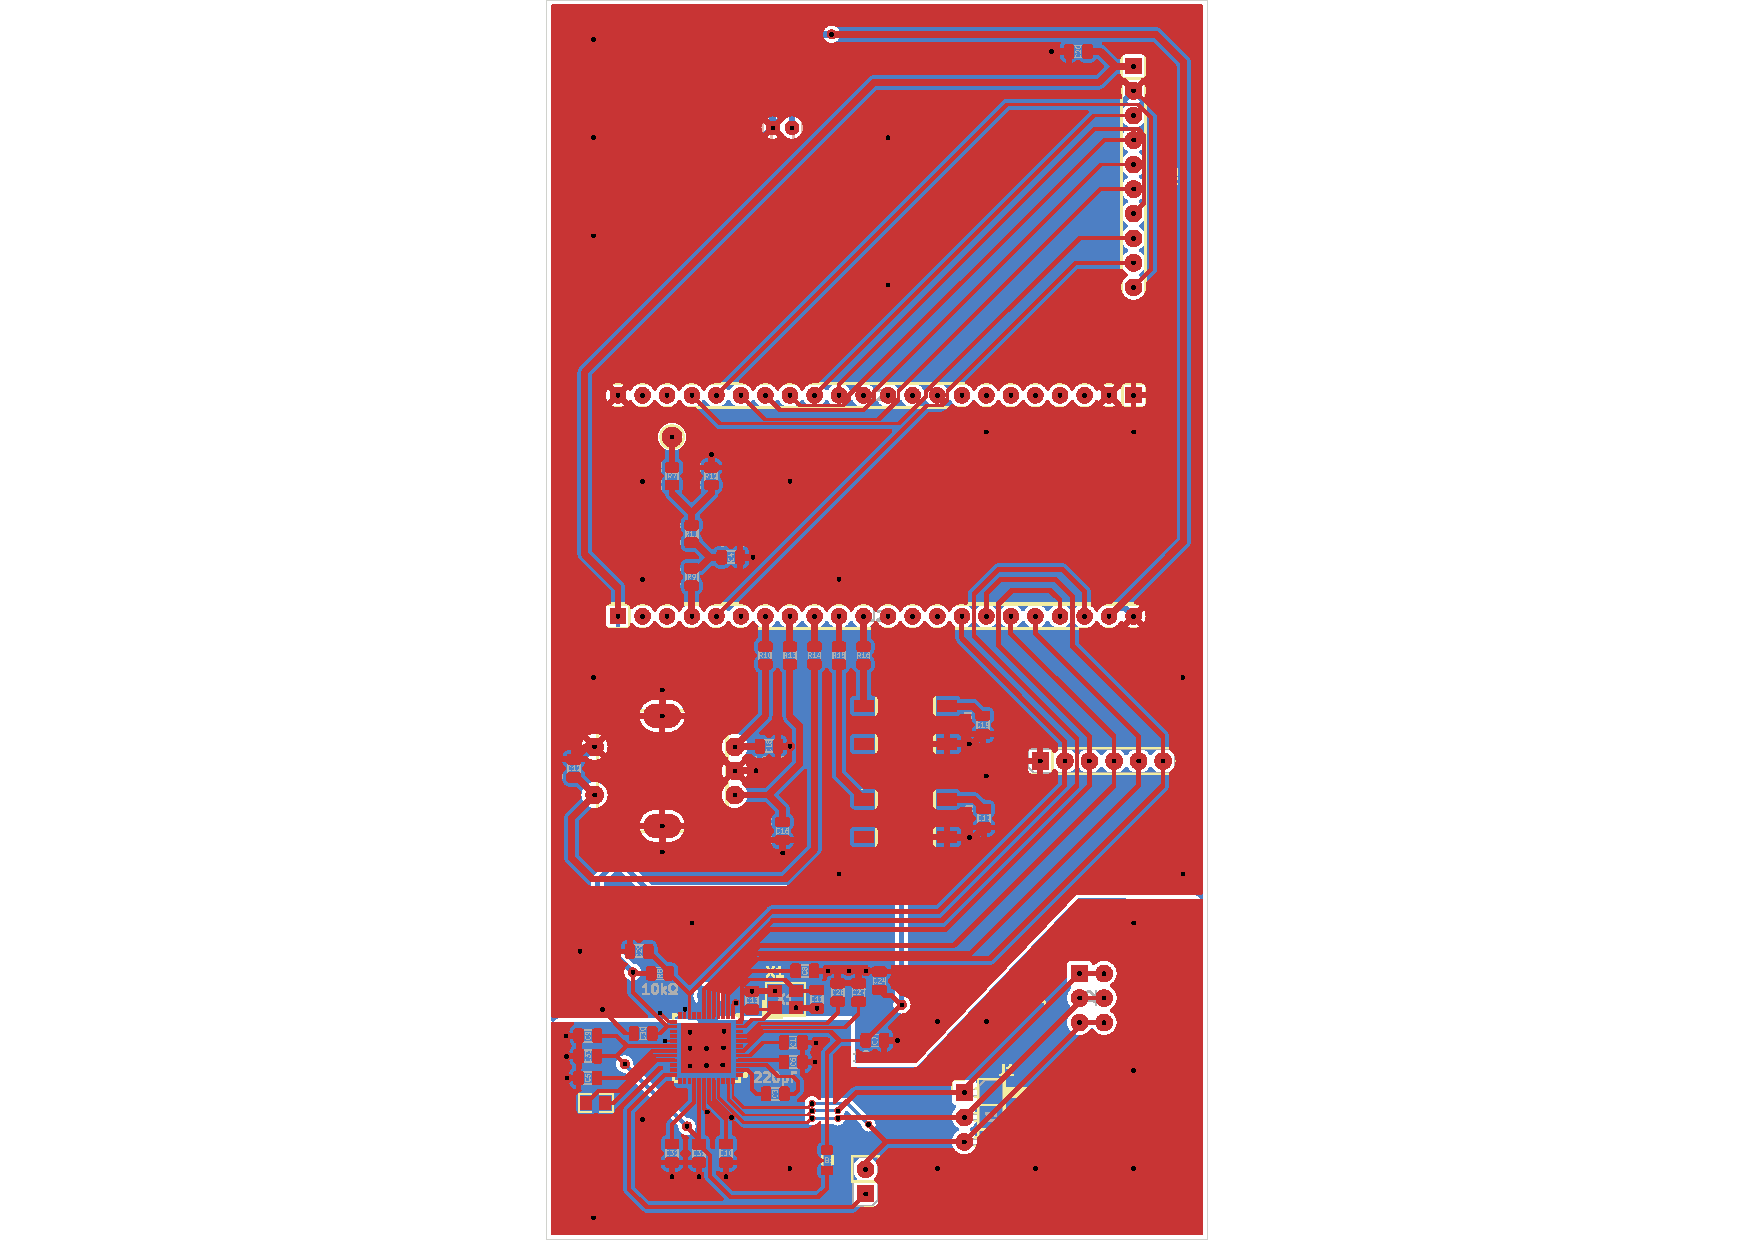
\includegraphics[trim=265 0 265 0, clip, height=6.5cm]{figures/pcbexport.pdf}
\end{wrapfigure}
To combat this, the PCB was partitioned into an analog region and a digital
region, which are the lower and upper parts of the board respectively
(Figure~\ref{fig:hw_ground_partition}), with
all digital components and traces confined to the digital region.
Partitioning is effective because, at high frequencies such as those in
digital edges, the return current follows the path of least inductance and
flows in the ground copper directly beneath its own signal trace
\cite{ott2009emc, pithadia2013grounding}. In accordance with Analog Devices guidance, the analog and digital grounds should be joined through the
shortest possible connection \cite{pithadia2013grounding, adi_mt031}. This is done by stitching them together directly beneath
the AD5941, commonly called a star ground connection \cite{adi_mt031}. The
stitched bridge also serves as the crossing point for the SPI bus and the
reset and interrupt lines, so each signal retains a continuous return path
directly underneath it. If the two grounds had been fully separated and joined
only at a distant point, such as the power input, these return currents would
be forced around a large loop that acts as an antenna \cite{ott2001partitioning}.

At the sub-nanoampere currents estimated in Section~\ref{sec:dpv_applications}, leakage and interference on the working-electrode path can set the noise floor. The electrode lead used in testing was unshielded; however, it was kept short to minimise noise pickup. A spare analog ground pin beside the electrode interface allows a shielded cable to be terminated at the interface.

\subsection{Trace Widths}
\label{sec:hw_trace_widths}

Trace widths were checked with the IPC-2221 equations \cite{ipc2221} as implemented in the DigiKey calculator \cite{digikey_tracewidth}, for a \SI{10}{\celsius} rise in 1\,oz/ft\textsuperscript{2} external copper. The \SI{0.3}{\milli\metre} traces used for the AD5941 and display nets can carry \SI{1.0}{\ampere} and the \SI{0.6}{\milli\metre} supply traces \SI{1.65}{\ampere}, well above their design currents of \SI{10}{\milli\ampere}, \SI{33}{\milli\ampere} and \SI{1}{\ampere}. See Appendix~\ref{app:trace_width} for more information.

\section{Display and SD Card}
\label{sec:hw_display}

The DFRobot Fermion 1.8-inch TFT (DFR0928) was selected as the display because it meets requirements R4–R7 from Table~\ref{tab:requirements_whole_sys}. The Fermion was the only component in stock that met all the criteria. Additional information regarding the display is given in Appendix Table~\ref{tab:hw_display_specs}.

The display and the SD card share a single SPI bus, because the ESP32-S3 has only two general-purpose SPI controllers \cite{esp32s3_wroom2_ds}. This allows a full SPI bus to be dedicated to the AD5941, so that scans are minimally affected. The cost is that the display and the SD card cannot be used at the same time. This is avoided by buffering the samples in PSRAM and writing the file
only after the scan has finished.

\section{Power Management}
\label{sec:hw_power}

The power subsystem was chosen to meet the requirements of 8-hour working day battery
life, over-voltage and under-voltage protection, and affordable components.
The chosen components are the TP4056 charger with a DW01A protection IC, the
Pololu S9V11E2F5 step-up/step-down regulator producing \SI{5}{\volt}, and a
\SI{5000}{\milli\ampere\hour}, \SI{3.7}{\volt} single-cell LiPo battery. Their
main specifications are summarised in Table~\ref{tab:hw_power_specs}.

\subsection{Battery}
\label{sec:hw_battery}

To verify that the selected \SI{5000}{\milli\ampere\hour} battery fulfils the full-day operational requirement, the system's current was measured during idle, transmission over Wi-Fi and DPV measurements. The supply current was measured by powering the PCB at \SI{5}{\volt} from a Siglent SPD3303C bench supply and reading the output current from the supply. The SPD3303C has a current
readback resolution of \SI{10}{\milli\ampere} and an accuracy of
$\pm\SI{0.5}{\percent}$
\cite{siglent_spd3303c}, that is, about $\pm\SI{21}{\milli\ampere}$ at these
currents. The board draws $\SI{100}{\milli\ampere} \pm \SI{21}{\milli\ampere}$
at idle and $\SI{160}{\milli\ampere} \pm \SI{21}{\milli\ampere}$ while
transmitting over Wi-Fi. The idle current did not change when taking a DPV measurement. Taking \SI{160}{\milli\ampere} as the worst case, the power drawn from the
battery through the regulator ($\eta_\text{reg} \approx 0.9$) is
\begin{equation}
  P_\text{bat} = \frac{\SI{5}{\volt} \times \SI{160}{\milli\ampere}}
                      {\eta_\text{reg}}
               = \frac{\SI{0.80}{\watt}}{0.9}
               \approx \SI{0.89}{\watt},
  \label{eq:hw_pbat}
\end{equation}
and the run time is
\begin{equation}
  t_\text{run} = \frac{E_\text{bat}\,\eta_\text{reg}}{V_\text{out}\,I_\text{load}}
    = \frac{\SI{5}{\ampere\hour} \times \SI{3.7}{\volt} \times 0.9}
           {\SI{5}{\volt} \times \SI{160}{\milli\ampere}}
    \approx \SI{21}{\hour}.
  \label{eq:hw_runtime}
\end{equation}
Allowing for the measurement uncertainty, the run time with Wi-Fi
transmitting lies between \SI{18}{\hour} and \SI{24}{\hour}, and at idle
between \SI{28}{\hour} and \SI{42}{\hour}. Even the lower bound comfortably
meets R12, as well as R9--R11.

\subsection{Charging}
\label{sec:hw_charging}

The TP4056 is a linear constant-current, constant-voltage charger with a
\SI{4.2}{\volt} float voltage, which charges at up to \SI{1}{\ampere} \cite{tp4056_ds}. A full charge of the \SI{5000}{\milli\ampere\hour} cell was measured to take about \SI{6.5}{\hour}, longer than the \SI{5}{\hour} that capacity divided by current suggests, because the charger reduces the current in its final constant-voltage stage.

\subsection{Regulation}
\label{sec:hw_regulation}

The Pololu S9V11E2F5 covers the full battery voltage range with sufficient
output current, but it requires the addition of an external low-voltage
cutoff. An MT3608 boost converter was also considered, but was rejected after three of the modules tested proved faulty. The Pololu's \SI{700}{\milli\ampere} start-up current limit is sufficient for
the ESP32-S3 to boot, and its soft-start ramps the output up gradually
\cite{pololu_s9v11e2f5}. The regulator has a \SI{100}{\kilo\ohm} pull-up
resistor from its enable pin to $V_\text{IN}$; the enable pin turns the
regulator off below \SI{0.7}{\volt} and on above \SI{0.8}{\volt}
\cite{pololu_s9v11e2f5}. Connecting a \SI{33}{\kilo\ohm} resistor from the
enable pin to ground forms a divider that switches the regulator off at about \SI{2.8}{\volt}, as given in Equation~\eqref{eq:hw_cutoff}.

The divider draws about \SI{28}{\micro\ampere} continuously, which is
sufficiently low for this application.
\begin{equation}
  V_\text{off} = \SI{0.7}{\volt} \times
    \frac{\SI{100}{\kilo\ohm} + \SI{33}{\kilo\ohm}}{\SI{33}{\kilo\ohm}}
    \approx \SI{2.8}{\volt}
  \label{eq:hw_cutoff}
\end{equation}

The \SI{5}{\volt} output supplies the ESP32-S3 development board, whose on-board regulator provides the \SI{3.3}{\volt} rail for the whole PCB, including AVDD of the AD5941.
% CHECK: confirm this matches your board; if the 3.3 V comes from a regulator on your own PCB, name that part instead.
A design oversight was the choice to boost the voltage to \SI{5}{\volt} when
no component requires a \SI{5}{\volt} supply. A \SI{3.3}{\volt}
step-up/step-down regulator would have been more efficient. The large
\SI{5000}{\milli\ampere\hour} battery makes this loss affordable, although it
is not ideal.

\subsection{Input Decoupling}
\label{sec:hw_input_decoupling}

No single capacitor has a low impedance across the whole frequency range, so a
large capacitor for low frequencies is paired with a small one for high
frequencies \cite{adi_mt101}. Decoupling is required because high-frequency
noise couples through to the regulator output and must be kept out of the chip
\cite{adi_mt101}. A \SI{100}{\micro\farad} bulk capacitor is used at the
output of the boost regulator, which is the input to the PCB, to act as a
local charge reservoir. An additional \SI{100}{\nano\farad} capacitor shunts
high-frequency noise away from the PCB \cite{adi_mt101}.

\section{User Interface}
\label{sec:hw_ui}

The interface consists of two push buttons and a rotary encoder with an integrated push button. All are wired in an active-low configuration with \SI{10}{\kilo\ohm} hardware pull-up resistors. A capacitor on each line forms an RC filter with its pull-up, so on release the pin only reads high once the capacitor has charged past the ESP32-S3 input-high threshold of $0.75 \times V_{DD}$ \cite{esp32s3_ds}. This takes $t = RC\ln 4 \approx 1.39\,RC$.

The push buttons use \SI{100}{\nano\farad} (\SI{1.4}{\milli\second}) to absorb contact bounce \cite{allpcb_debounce}, and the encoder lines use \SI{10}{\nano\farad} (\SI{0.14}{\milli\second}) so that fast rotation is not smeared; the remaining encoder bounce, which can last up to \SI{2}{\milli\second} \cite{alps_ec11}, is rejected by the quadrature decoder in firmware.

The OpenStat has two user interfaces, shown in Figure~\ref{fig:interface}. On the device, the rotary encoder selects and edits the scan parameters of Table~\ref{tab:sw_params}, the push buttons start and stop a scan, and the display shows the voltammogram as it is measured. The web interface offers the same parameters, a live voltammogram and a list of stored scans that can be downloaded. If the device cannot join a known Wi-Fi network, it starts its own access point, so that a phone or laptop can connect to it in the field (Section~\ref{sec:sw_toplevel}).

\begin{figure}[htbp]
  \centering
  \caption{OpenStat user interfaces. (a) Physical interface, shown connected to the Randles test circuits. (b) Web interface displaying a live voltammogram.}
  \label{fig:interface}
  \begin{minipage}[b]{0.38\textwidth}
    \centering
    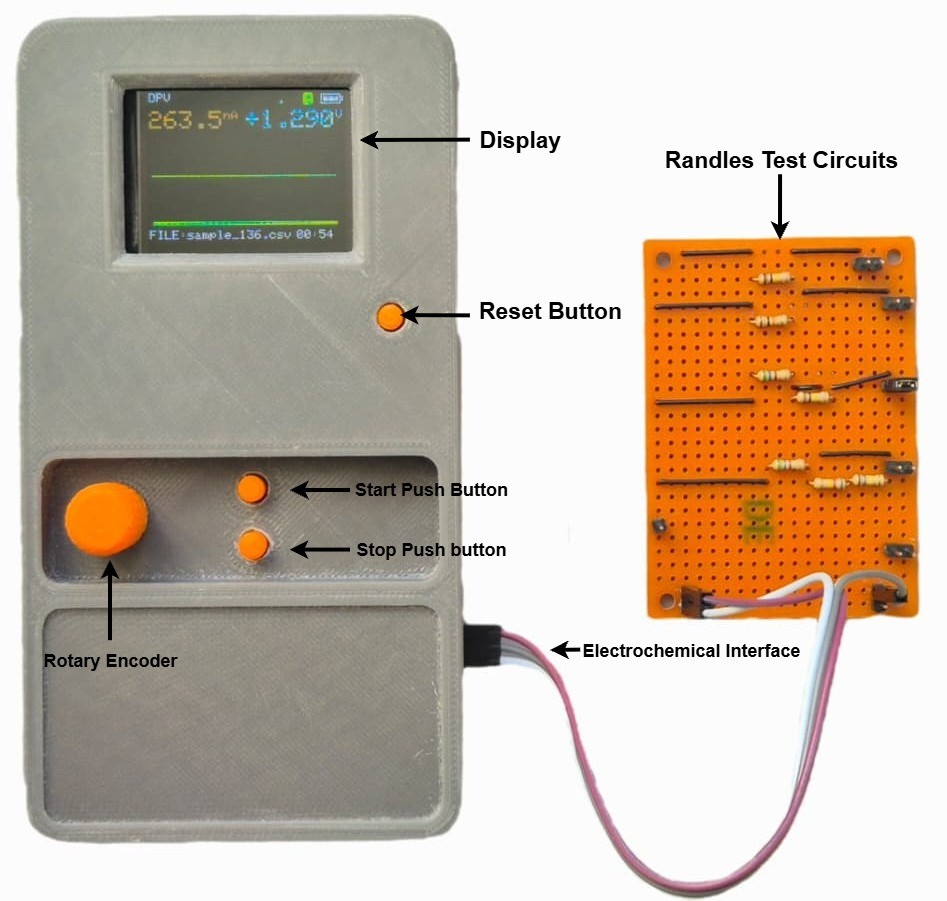
\includegraphics[width=\linewidth]{figures/sweep_136_lab.jpg}\\
    (a)
  \end{minipage}
  \hfill
  \begin{minipage}[b]{0.58\textwidth}
    \centering
    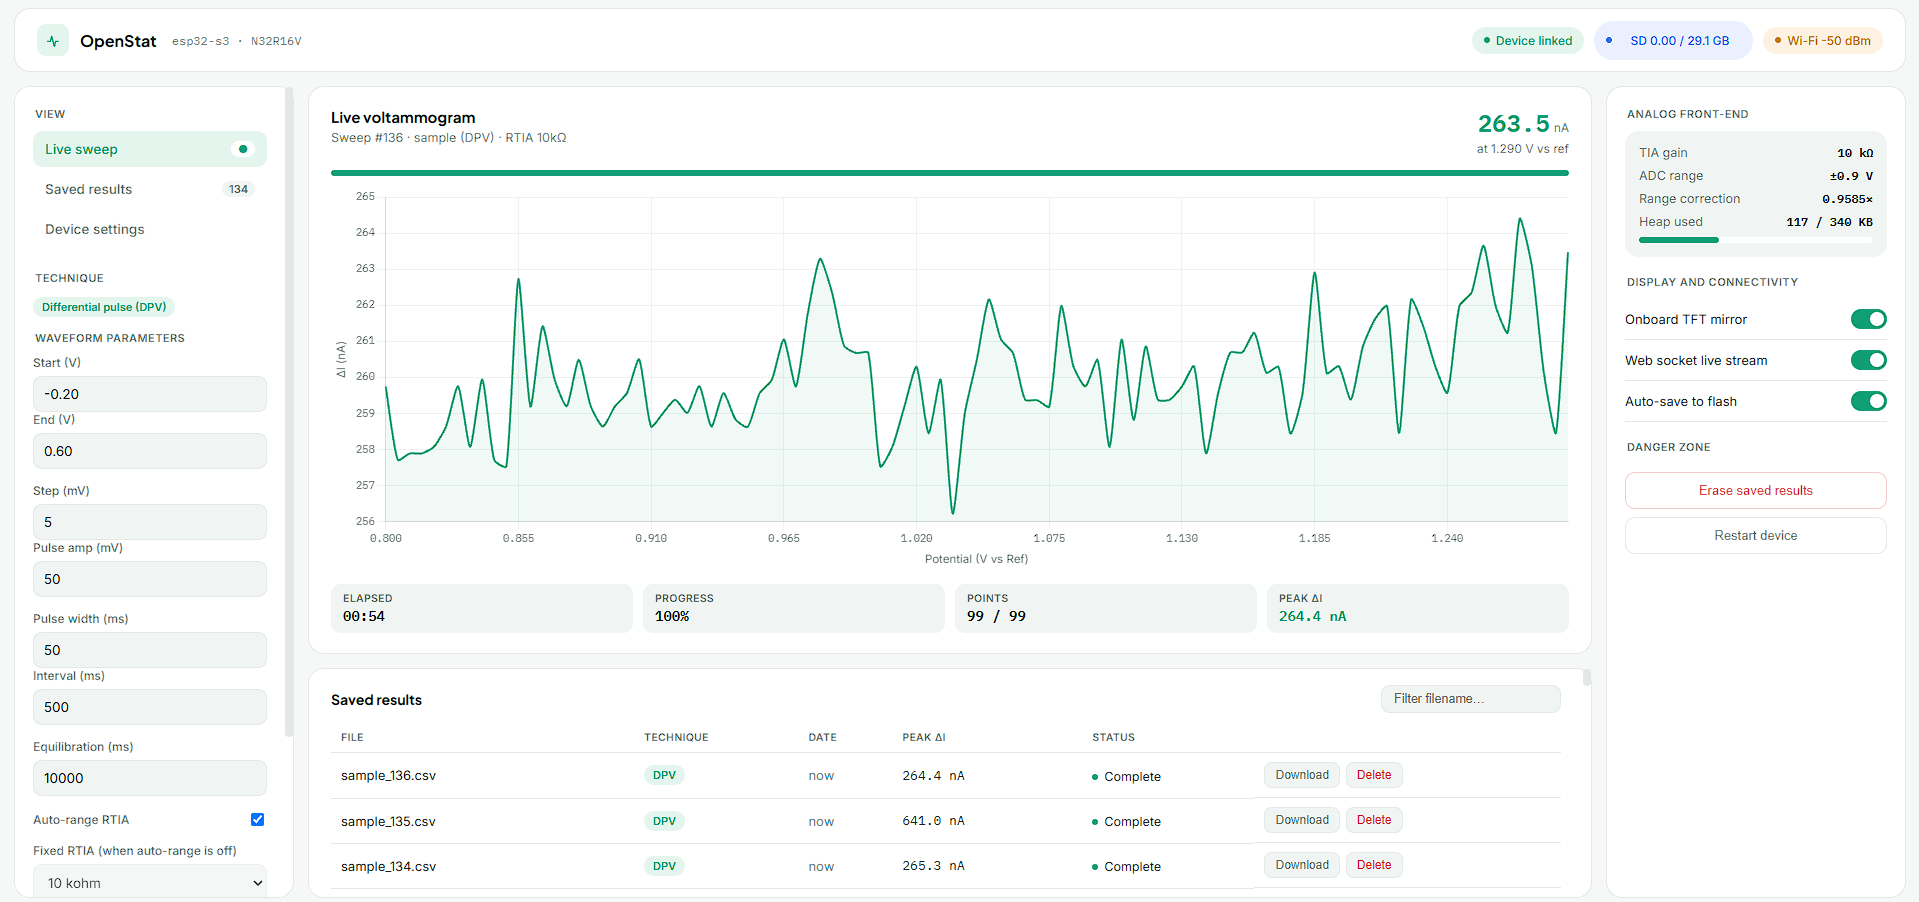
\includegraphics[width=\linewidth]{figures/sweep136.png}\\
    (b)
  \end{minipage}
\end{figure}